%
% latex-sample.tex
%
% This LaTeX source file provides a template for a typical research paper.
%

%
% Use the standard article template.
%
\documentclass{article}

\usepackage{titling}


\usepackage{float}
                   % collegamenti ipertestuali

\usepackage[babel]{csquotes}

\usepackage{lastpage}
\usepackage{fancyhdr}
\usepackage{booktabs,tabularx}
\usepackage{makeidx}
\usepackage{fixltx2e}
%\usepackage{hyperref}


% The geometry package allows for easy page formatting.
\usepackage{geometry}
\geometry{letterpaper}

% Load up special logo commands.
\usepackage{doc}

% Package for formatting URLs.
\usepackage{url}
\usepackage[utf8]{inputenc}
\usepackage{caption}

% Packages and definitions for graphics files.
\usepackage{graphicx}
\usepackage{epstopdf}
\usepackage{stfloats}
\usepackage{adjustbox} 
\usepackage[colorlinks, linkcolor = blue, urlcolor = blue]{hyperref}
\DeclareGraphicsRule{.tif}{png}{.png}{`convert #1 `dirname #1`/`basename #1 .tif`.png}

\usepackage[final]{pdfpages}
\usepackage{shellesc}

\usepackage{tabularx,pbox}
\usepackage{here}


%
% Set the title, author, and date.
%
\title{\LARGE \textbf{Titolo appropriato}}
\author{Anna Bonaldo \and Vassilikì Menarin }
\date{\small {Email: anna.bonaldo@studenti.unipd.it vassiliki.menarin@studenti.unipd.it }}

\def\code#1{\texttt{#1}}

%
% The document proper.
%
\begin{document}
	
	% Add the title section.

	\maketitle
	
	\textbf{\textit{Abstarct} - Write something interesting here}

	
	\section{Introduction}
	\subsection{Work Staling Scheduler}
	Work stealing is a scheduling strategy designed to efficiently manage a dynamically multithreaded computation using a fixed number of processors. The work stealing scheduler bounds the number of concurrently active threads within a limit, thus affecting the memory requirements too. This causes an improvement in the execution time and memory usage. Moreover, the scheduler tries to mantain related threads on the same processor, minimizing the communication between different threads.
	Work stealing differs from work sharing because underutilized processors take the initiative, without relying soley on the scheduler: each processor owns a deque and, when it-s empty, it tries to steal work from others. The number of migrations is lower in work stealing, because it is done only when absolutely necessary.
	
	We built a work stealing scheduler that runs a Quick Sort application. We performed some analysis on the results, comparing the clock-time and CPU time for a work stealing and a sequential scheduling, searching for a set of paramentrs that minimizes wall-clock time.
	
	\section{Our work}
	We developed a work-stealing scheduler and a Quick-Sort application using Java 8. The main routine takes three parameters, and we tried assigning different values to them to find a set that minimizes wall-clock time when compared to sequential sorting. For more information about the parametrs used, see \href{analysis}{Section 3}. 
	The classes that implement the algorithm are \code{Scheduler}, \code{Tasklet} and \code{QuickSort} We then use \code{BatchQuickSortExecutors}, \code{IOFromCSVFile} and \code{Statistics} to efficiently gather and compute data.
	Details on the analysis performed can be found in \href{analysis}{Section 3}.
	
	\subsection{\code{Scheduler}}
	The work stealing scheduler is implemented using the \code{WorkstealingScheduler} class, which implements the \code{Scheduler} interface.
	The \code{WorkstealingScheduler} class contains a private \code{ServerThread[]} array named \code{servers}. The array represents the number of servers available.
	\code{ServerThread} is private inner class. 
	
	\paragraph {\code{ServerThread}}
	Each server is represented using a \code{ServerThread}. Each server has the fields:
	\begin{itemize}
		\item \code{private int myIndex}: the identifier of the server;
		\item \code{public ConcurrentLinkedDeque<Tasklet> deque}: each server has a deque to store the tasklets it needs to run. When dealing with its own deque, a server always adds and polls from the bottom of the deque;
		\item \code{private Stack<Tasklet> stack}: the stack stores the Tasklet the server is currently running.
	\end{itemize}
	The \code{ServerThread} class implements \code{Runnable}, and its two most important methods are:
	\begin{itemize}
		\item \code{public void run()}: defines the standard behaiour of the server. If the server's deque is void, the server calls the steal method; otherwise it polls the last Tasklet from the bottom of the deque, pushes it into the stack and then executes it;
		\item \code{public void steal()}:hagving its own deque empty, the server tries stealing Tasklets from the top of someone else's deque. If the steal is successful the server may proceed with the Tasklet execution.
	\end{itemize} 
	
	\subsection{\code{Tasklet}}
	\code{Tasklet} is an abstarct class designed to recursively perform a task. We mainly use the \code{QSortTasklet} class.
	
	\paragraph{\code{QSortTasklet}} This class was designed to recurively perform Quick Sort.Its most notable fields are:
	\begin{itemize}
		\item \code{public final int start, end} which are necessary to perform Quick Sort; 
		\item \code{private ConcurrentLinkedDeque<Tasklet> originDeque} keeping a reference to the deque the Tasklet was piqued from we can add one there one child while we execute the other;
	\end{itemize}
	
	As for its methods, since \code{QSortTasklet} extends \code{RecursiveAction}, it implements \code{compute()}.
	\begin{itemize}
		\item \code{public void compute()}: it's the main method of the class. It checks the size of the array or portion of array to sort and it confronts it with \code{cutOff}. If the size exceeds the cutoff we recursively call compute, otherwise we sort the remaining array sequentially. 
	\end{itemize}
	
	\subsection{The QuickSort class}
	It contains the \code{main} and the methods necessary to perform Quick Sort, \code{public void sequentialSortArray (int[] array, int left, int right)} and \code{public int partition (int arr[], int left, int right))}.
	
	\section{Analysis performed}\label{analysis}
	The work-stealing scheduler module takes as input three different execution parameters: 
	\begin{itemize}
		\item \code{arraySize}: sets the size of the array tp sort;
		\item \code{numServers}: sets the number of servers;
		\item \code{cutOff}: sets the array size under which to perform sequential sorting and it is used to improve the performances of the work stealing scheduler.
	\end{itemize}
		
	All these parameters affects the concurrent ordering execution time, and the relative speed-up on the sequential one.
	On each run, the array is copied and sorted twice, once completely sequentially, and once using the specified parameters. We collected different data searching the set of parameters that maximizes the speed-up.
	In order to evaluate the speed-up, we focused on wall-click time, which is the actual time taken just before and after sorting the array. The speed up reported is obtained dividing the concurrent clock time by the sequential one.
	
	\subsection{Results of analysis}
	
	We performed a series of analysis to determine the best set of parameters to maximize the speed up.
	
	\paragraph {Selecting the best number of servers} First we tried to determine the optimal number of servers. We set the cutoff at 100 considered arrays from $10^{5}$ to 5 x $10^{5}$. For each size we executed the program 5 times and computed then considered the average value. We tried using 5, 10, 15, 20, 25 and 30 servers.
	Using 10, 15 and 20 severs we always had a speed-up, so we chose between them the one with the better results. We concluded that the best number of servers with our data was 20.
	The following Figures show our results, while the detailed data can be found in the Appendix.
	
	\begin{figure*}[!h]
		\centering
		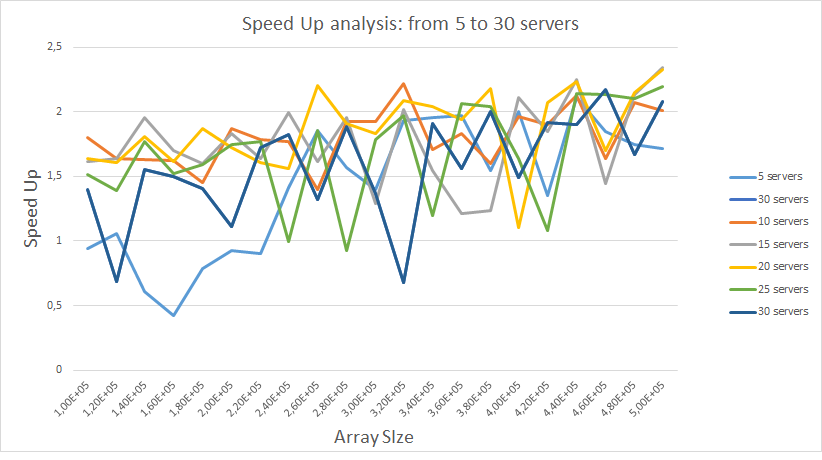
\includegraphics[width=0.8\linewidth]{imgs/SpeedUp5-30servers.png}
		\caption{Speed up with cutoff=100 and different sizes and servers}				
		\label{fig:SU01}
	\end{figure*}

	\begin{figure*}[!h]
		\centering
		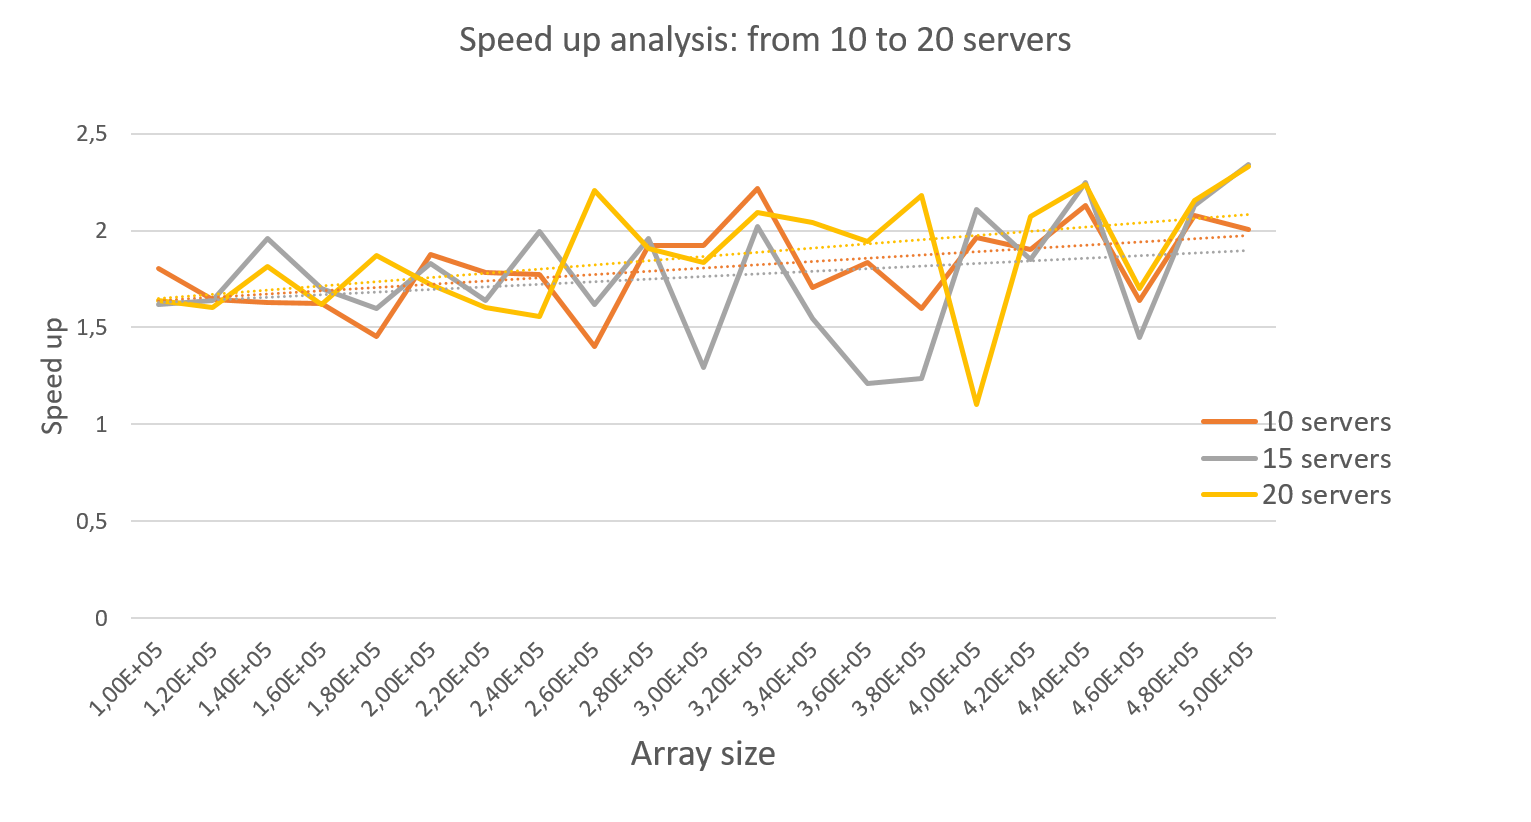
\includegraphics[width=0.8\linewidth]{imgs/SpeedUp10-20servers.png}
		\caption{Speed up with cutoff=100 and different sizes and servers}				
		\label{fig:SU02}
	\end{figure*}

	\paragraph {Selecting the best cut-off}
	We performed some analysis to see how a different cut-off affects the performance. We tried different cut-off values on different arrays, keeping the servers' number at 20. First we tested cut-off values ranging from 50 to 5000 with a step of 50 in an array with 1000000 and then 5000000 elements. The detailed results can be find in \href{CO1}{Appendix B1}.
	Figure 3 shows the speed-up obtained in the two arrays depending on the different cut-offs.
	
	\begin{figure*}[!h]
		\centering
		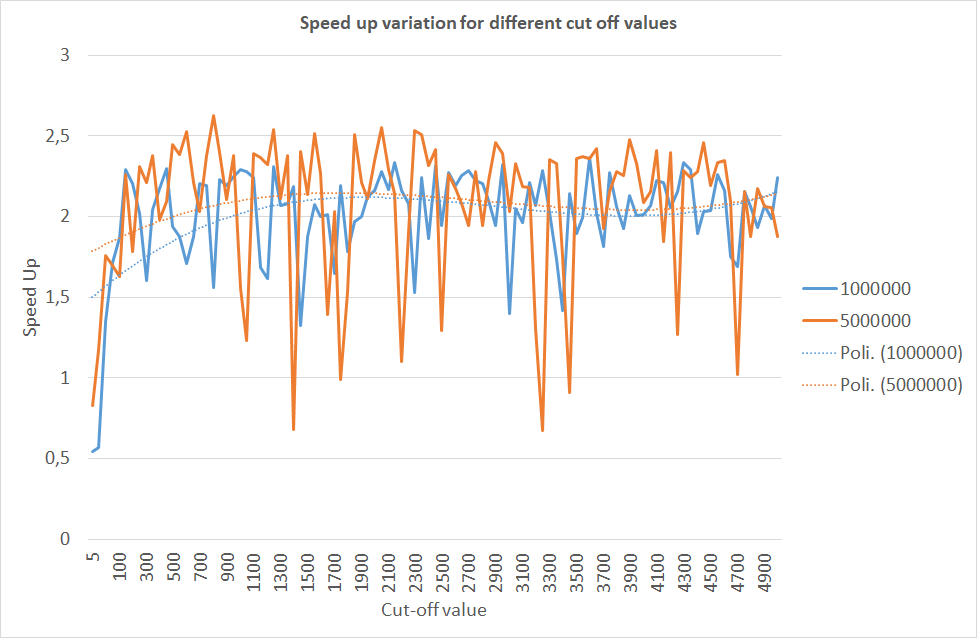
\includegraphics[width=0.8\linewidth]{imgs/SpeedUpForDifferentCutOff100-500mila.png}
		\caption{Speed-up on different two different arrays with 20 servers and varying cut-off values}				
		\label{fig:CO01}
	\end{figure*}
	
	After this first analysis we focused on some selected cut-off values: 50, 100, 500, 1000, 5000, 10000, 50000. 
	While the detailed data can be found in \href{CO2}{Appendix B2}, Figure 4 shows the speed-up for the best values obtained during analysis.
	
	
	\begin{figure*}[!h]
		\centering
		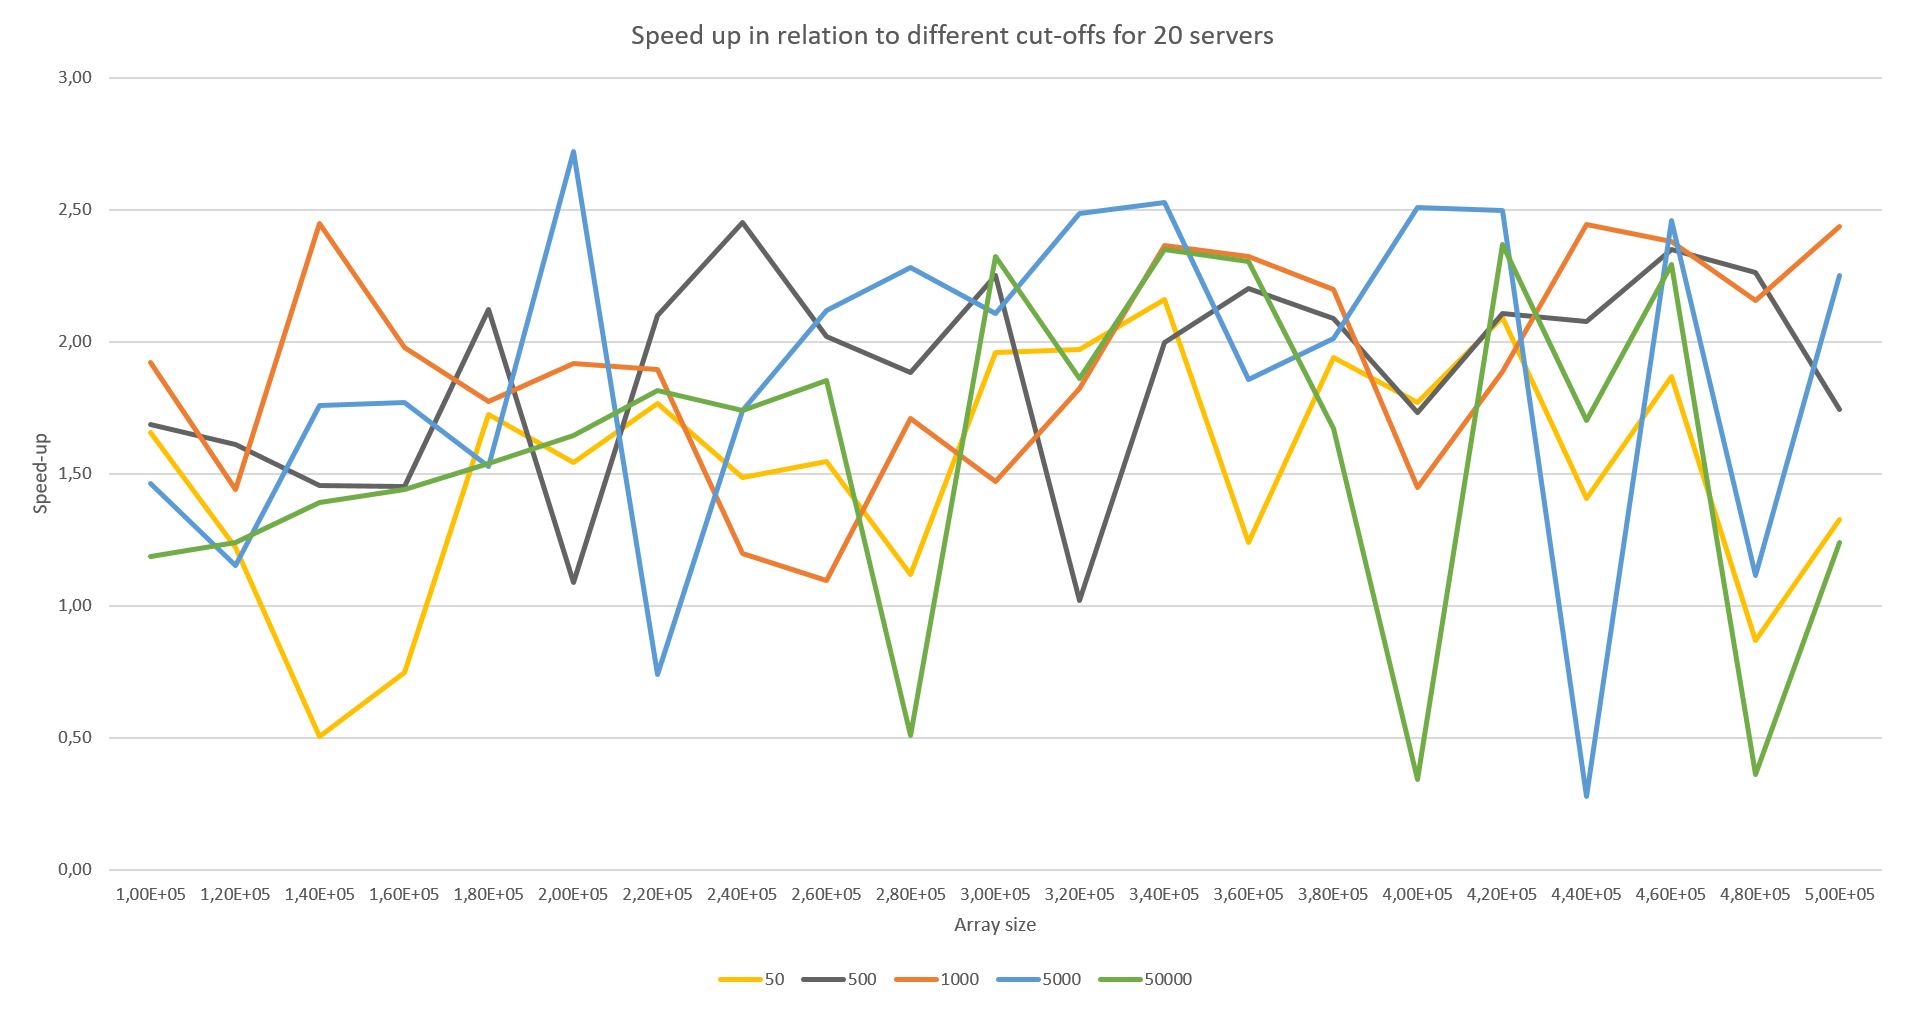
\includegraphics[width=0.8\linewidth]{imgs/CutOffs01.png}
		\caption{A simple program example}				
		\label{fig:CO02}
	\end{figure*}

	Figure 5 and 6 show the performances using the selected cut-off values after 5 executions. We determined that, with our data, 1000 was the best cut-off.	

	\begin{figure*}[!h]
		\centering
		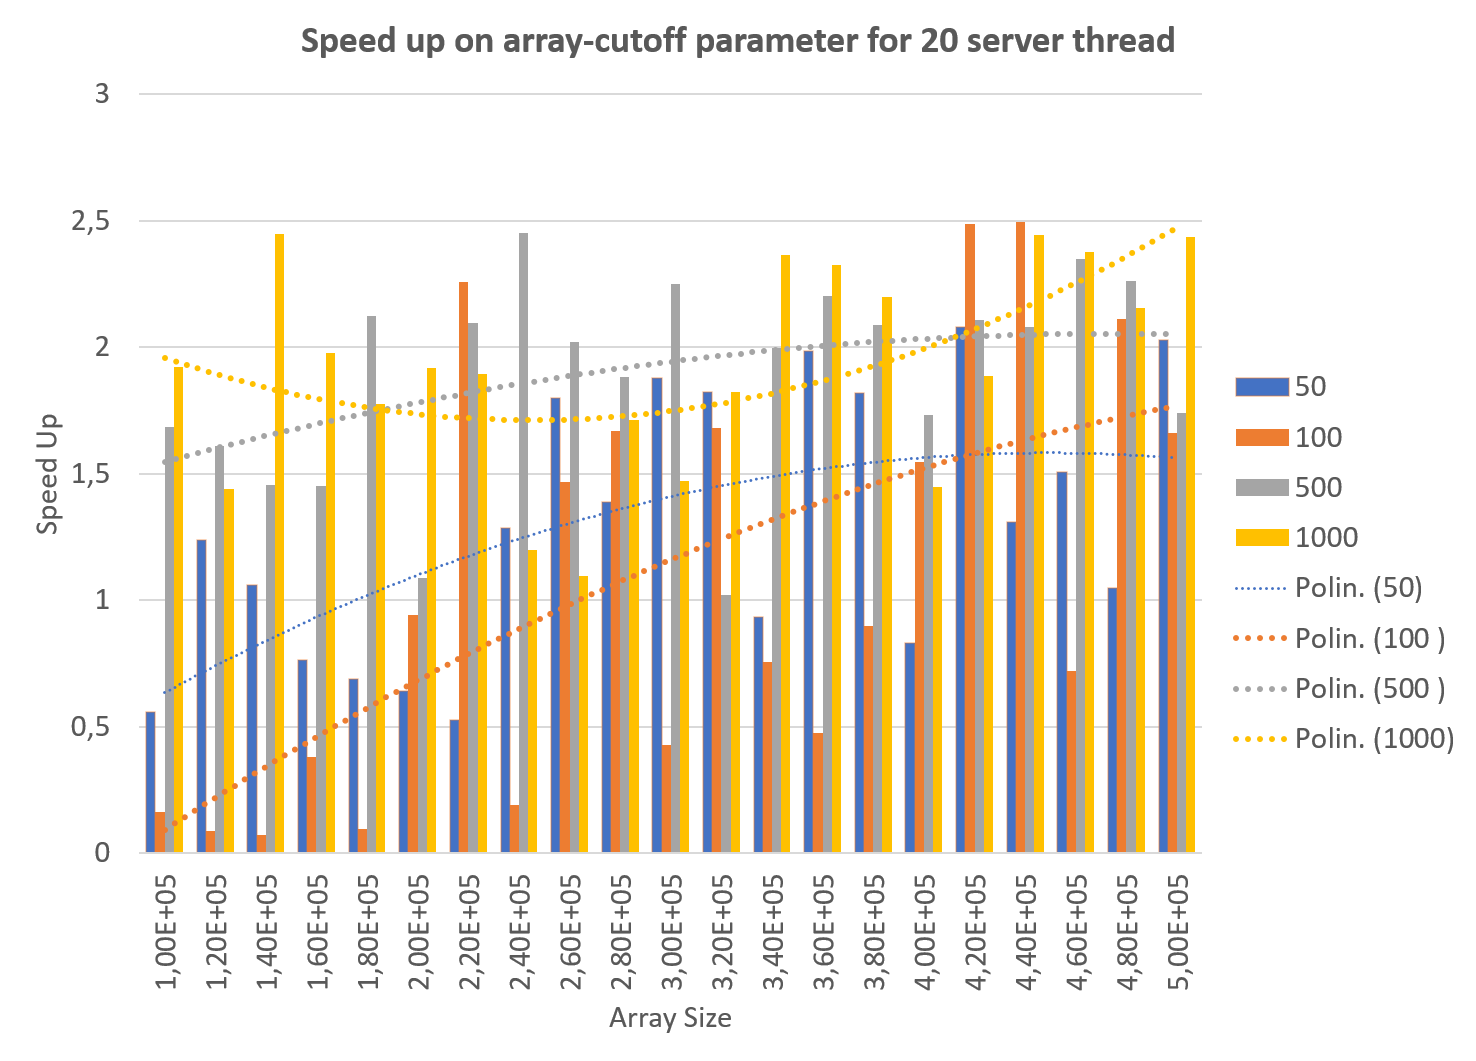
\includegraphics[width=0.8\linewidth]{imgs/hist01.png}
		\caption{A simple program example}				
		\label{fig:CO03}
	\end{figure*}

	\begin{figure*}[!h]
		\centering
		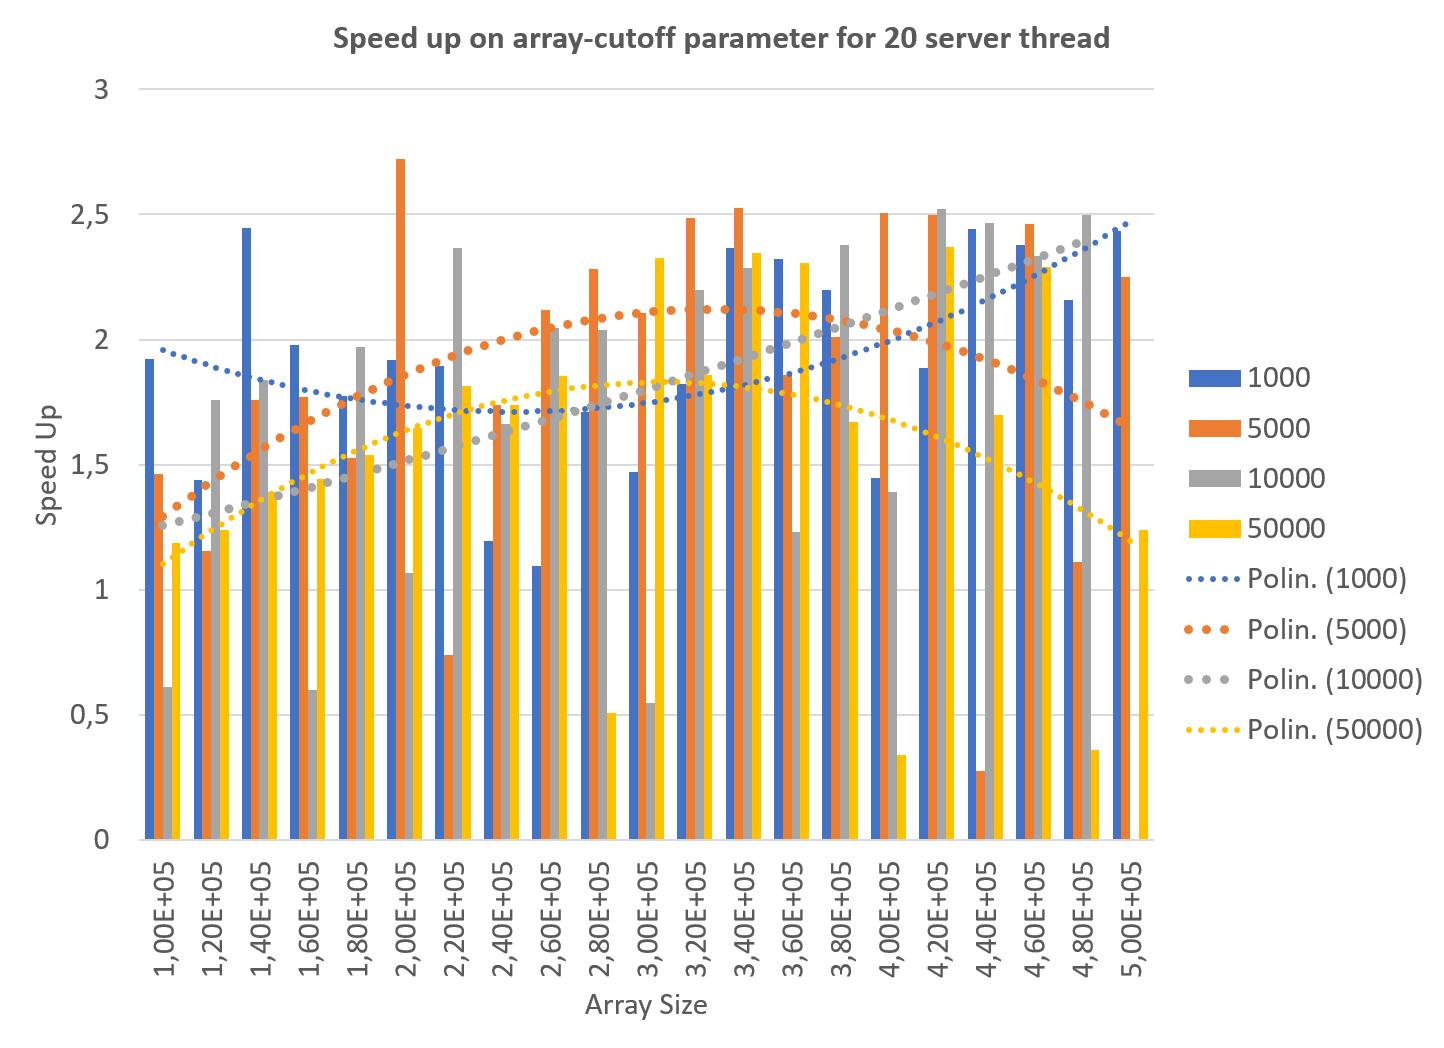
\includegraphics[width=0.8\linewidth]{imgs/hist02.png}
		\caption{A simple program example}				
		\label{fig:CO04}
	\end{figure*}

\clearpage

\section{Conclusions}
	In the tests we performed the work stealing scheduler showed better performances compared to sequential sorting.
	Given the range of array sizes we worked with we determined that the best values for number of servers and cutoff are 20 servers and a cutoff at 10000. 
	We run the program using this values and as, expected, the execution time was better using the work stealing algorithm.
	Figure 7 shows the comparison between the two algorithm with the parameters selected.	
			
	\begin{figure*}[!h]
		\centering
		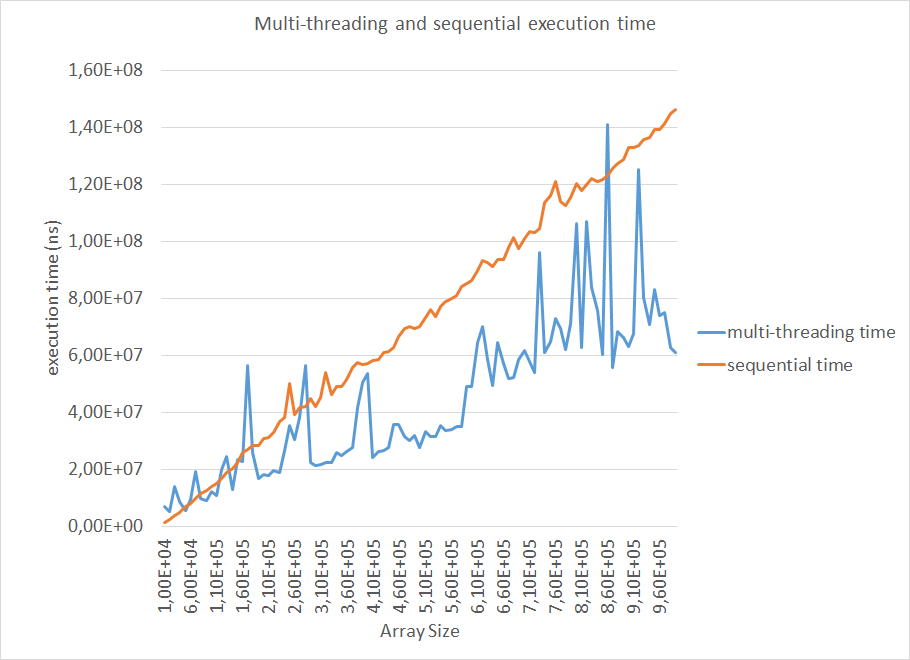
\includegraphics[width=0.8\linewidth]{imgs/seqVSmultithreading.png}
		\caption{Work stealing (with 20 servers and a cutoff value of 1000) and sequential sorting performances}				
		\label{fig:program}
	\end{figure*}

	Finally, we plotted the average number of stolen tasks (Figure 8). With a fixed number of servers, the number of stolen tasks increases with the size of the array. At a certain point it drops, because the servers are too busy to actually steal from others. The peak in stolen tasks coincides in a peak in performance.
	
	\begin{figure*}[!h]
		\centering
	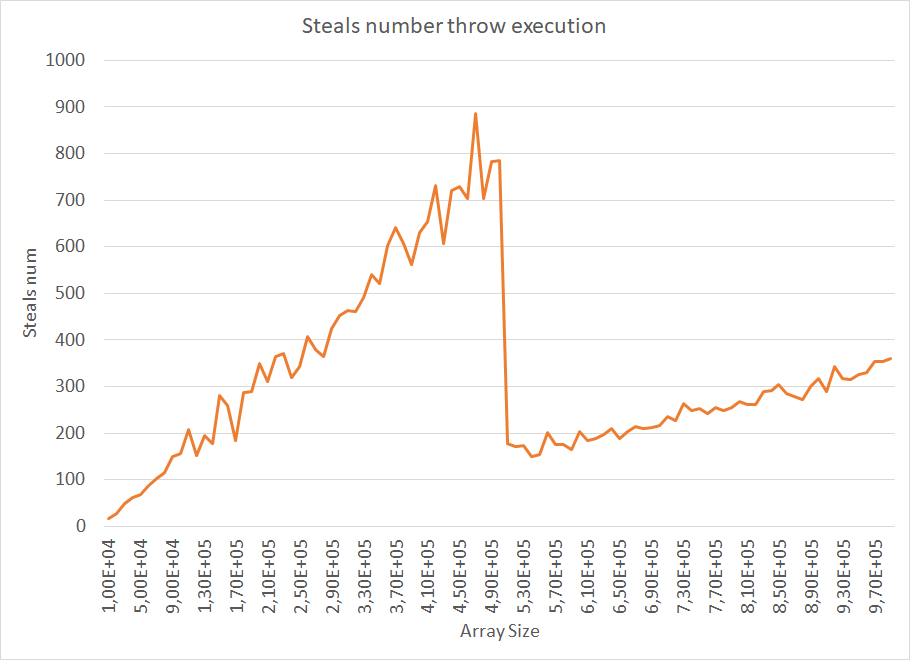
\includegraphics[width=0.8\linewidth]{imgs/stealsNum20servers1000cutoff.png}
		\caption{Number of stolen tasks with 20 servers and cutoff=1000}
		\label{fig:starve}
	\end{figure*}

%\newpage

\onecolumn
\appendix

%\immediate\write18{pdfcrop imgs/steals+multithreadVSseq.pdf}

\section{Speed-up in relation to the number of servers}
The table shows data collected while searching for an optimal number of servers. Green cells highlight the executions in which the work stealing algorithm had a better clock-time.

\begingroup
\centering
\hspace*{-1.5in}
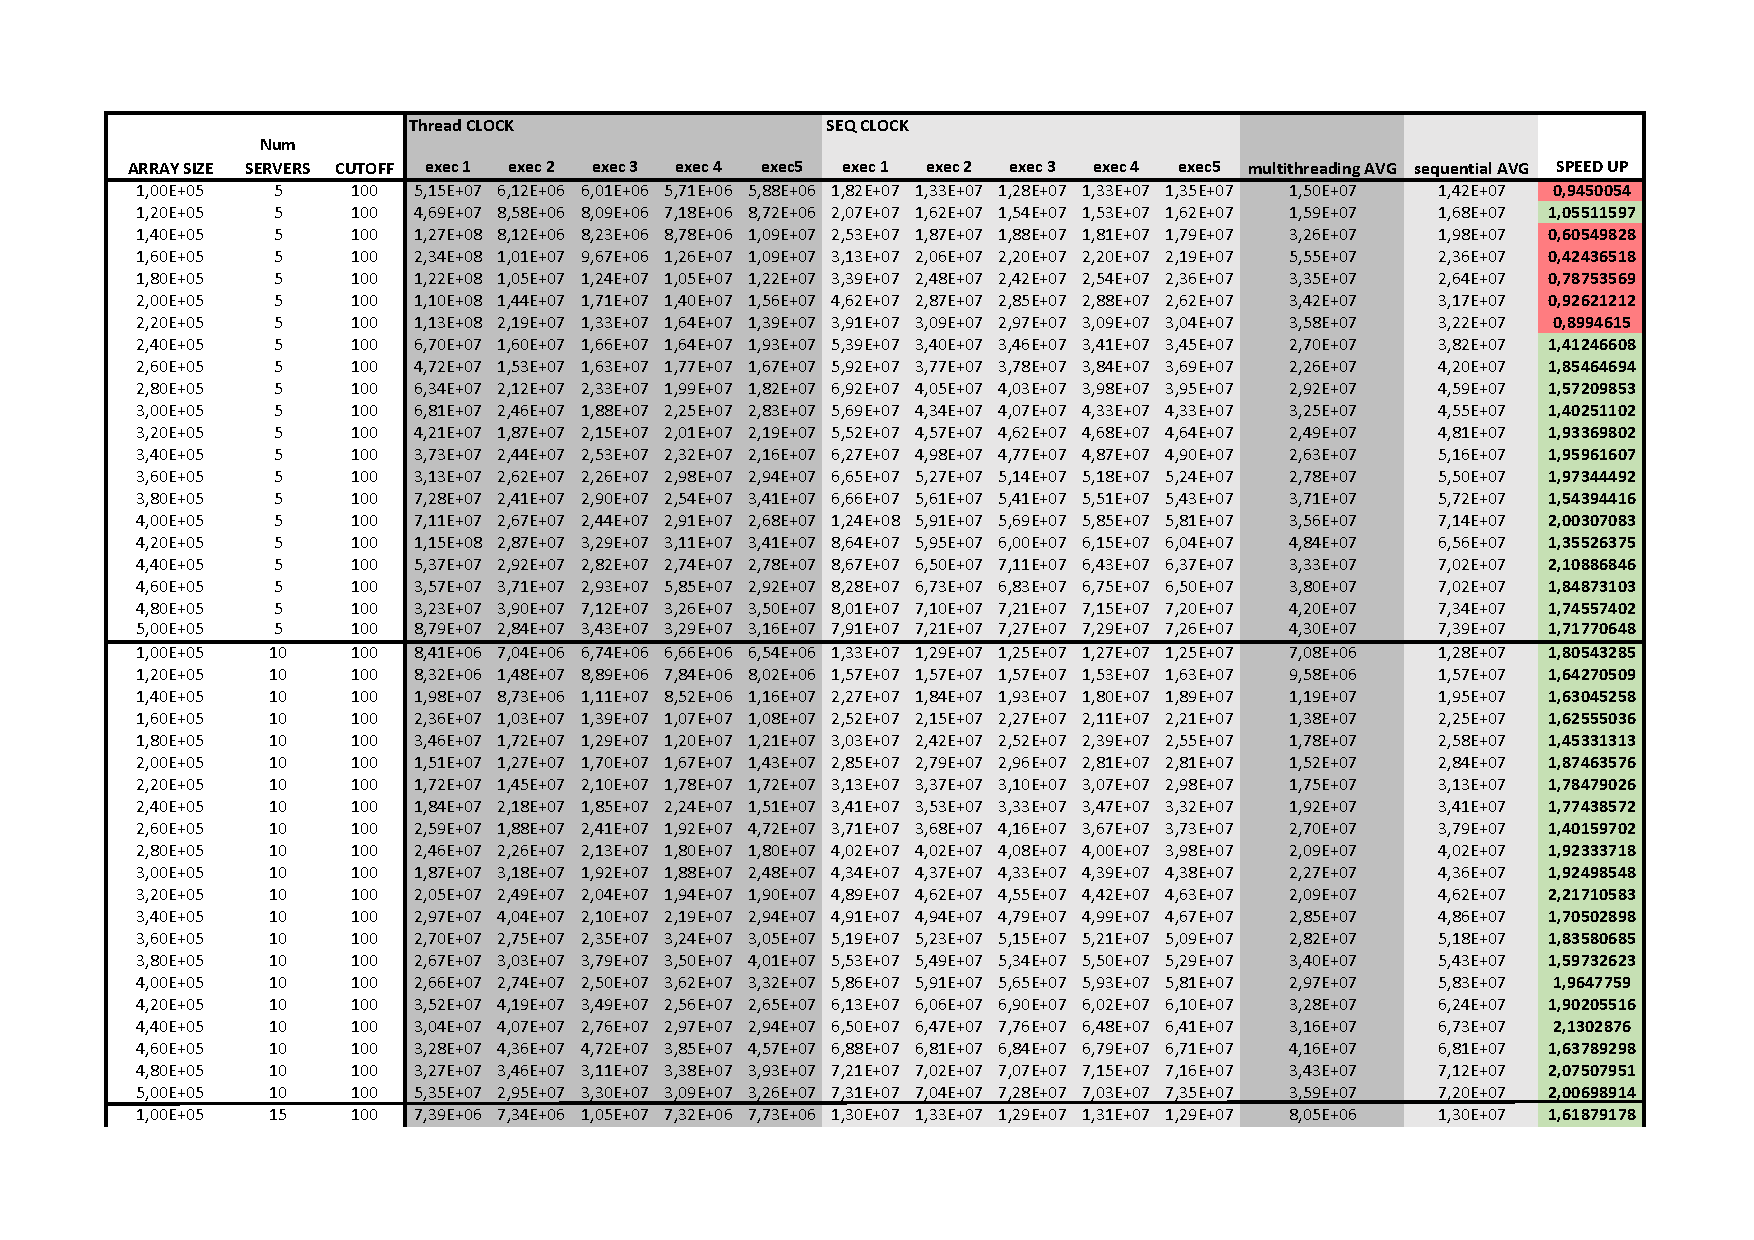
\includegraphics[page=1, width=1.5\linewidth]{imgs/ServerNumAnalysis.pdf}

\newpage
\hspace*{-1.5in}
\includegraphics[page=2, width=1.5\linewidth]{imgs/ServerNumAnalysis.pdf}%

\newpage
\hspace*{-1.5in}
\includegraphics[page=3, width=1.5\linewidth]{imgs/ServerNumAnalysis.pdf}%
\endgroup


\clearpage

\section{Cut-off analysis}
\subsection{Fine-grained analysis}\label{CO1}
We search for the best speed-up trying cut-off values ranging from 50 to 5000, first in an array with 1000000 and then 5000000 elements. The green cells highlight cut-off values above the average.

\begingroup
\centering
\vspace*{-0.3in}
\hspace*{-0.5in}
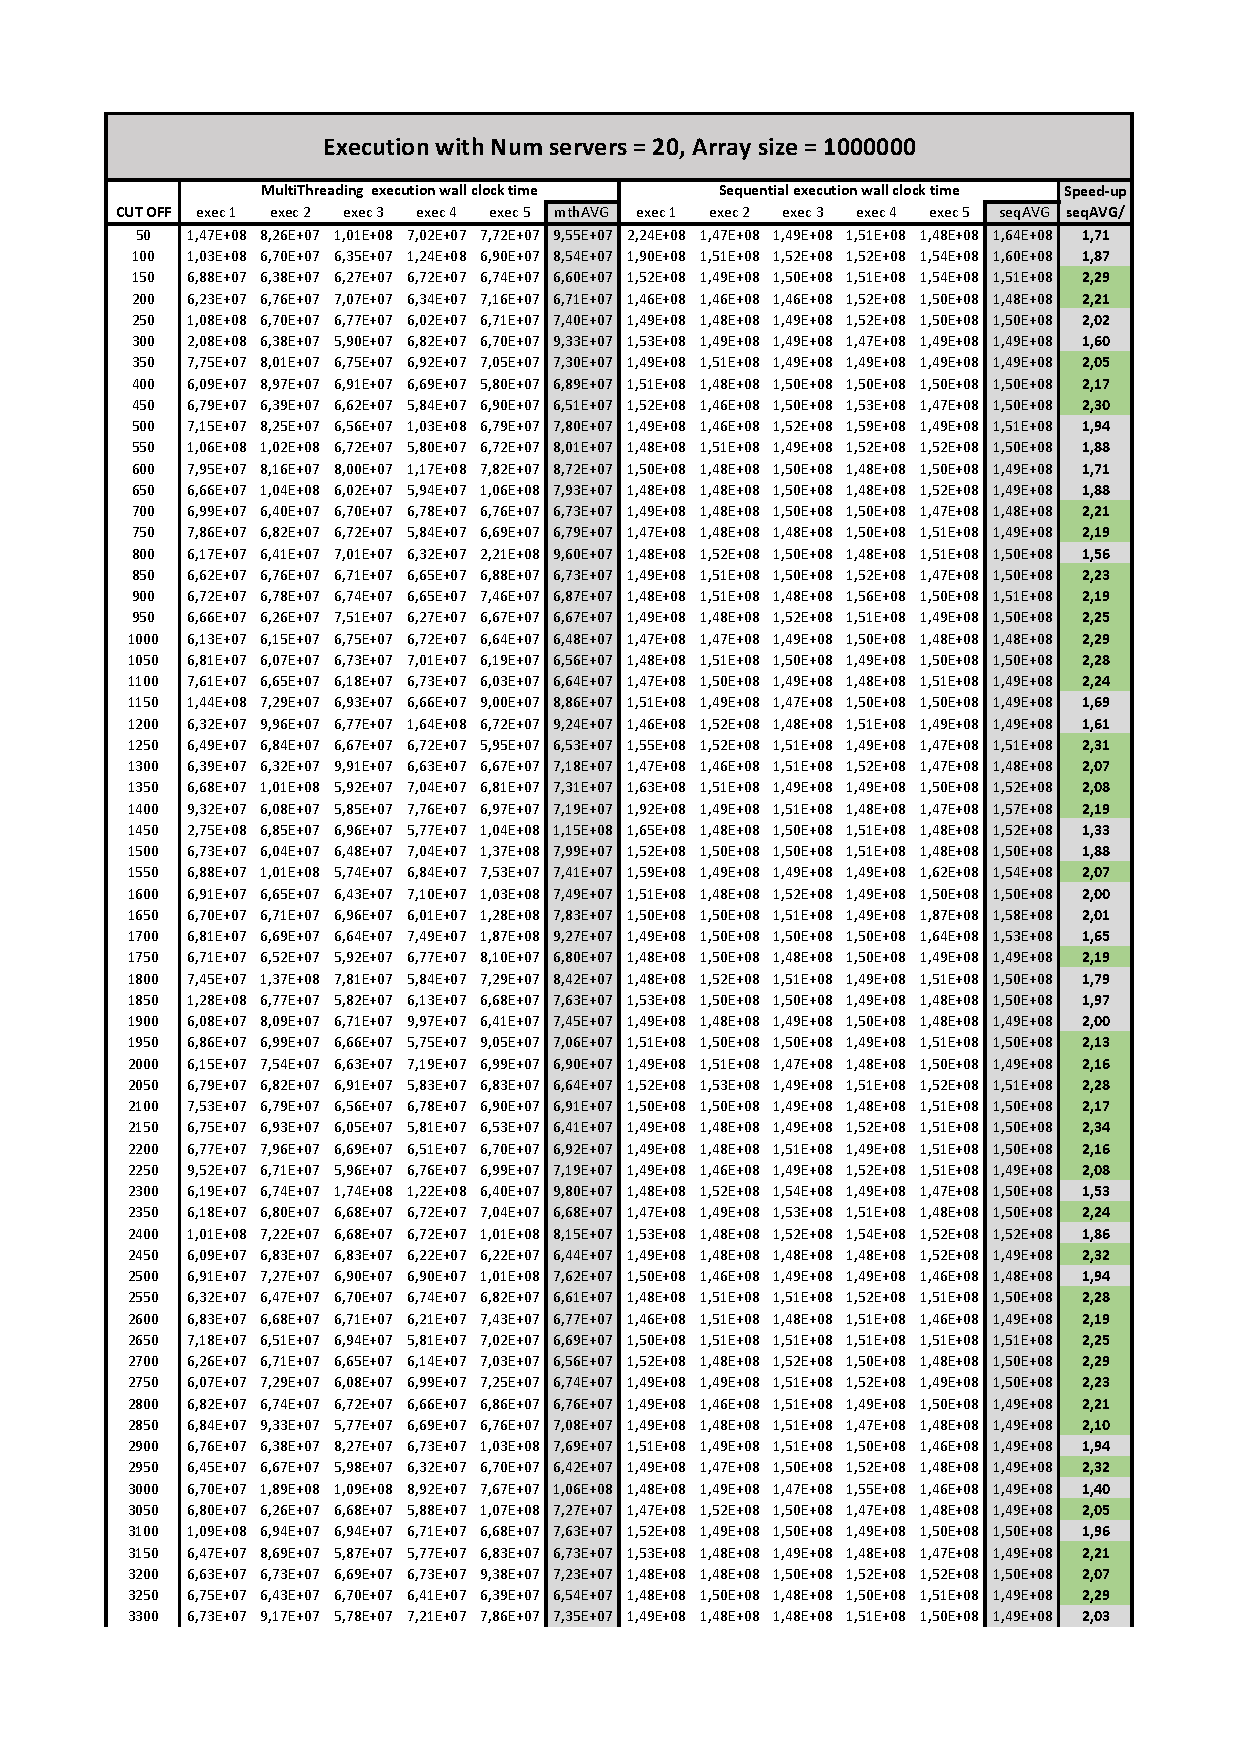
\includegraphics[page=1, width=0.9\linewidth]{imgs/CutOffAnalysis01.pdf}

\clearpage
\centering
\includegraphics[page=2, width=0.9\linewidth]{imgs/CutOffAnalysis01.pdf}
\endgroup

\begingroup
\centering
%\hspace*{-0.5in}
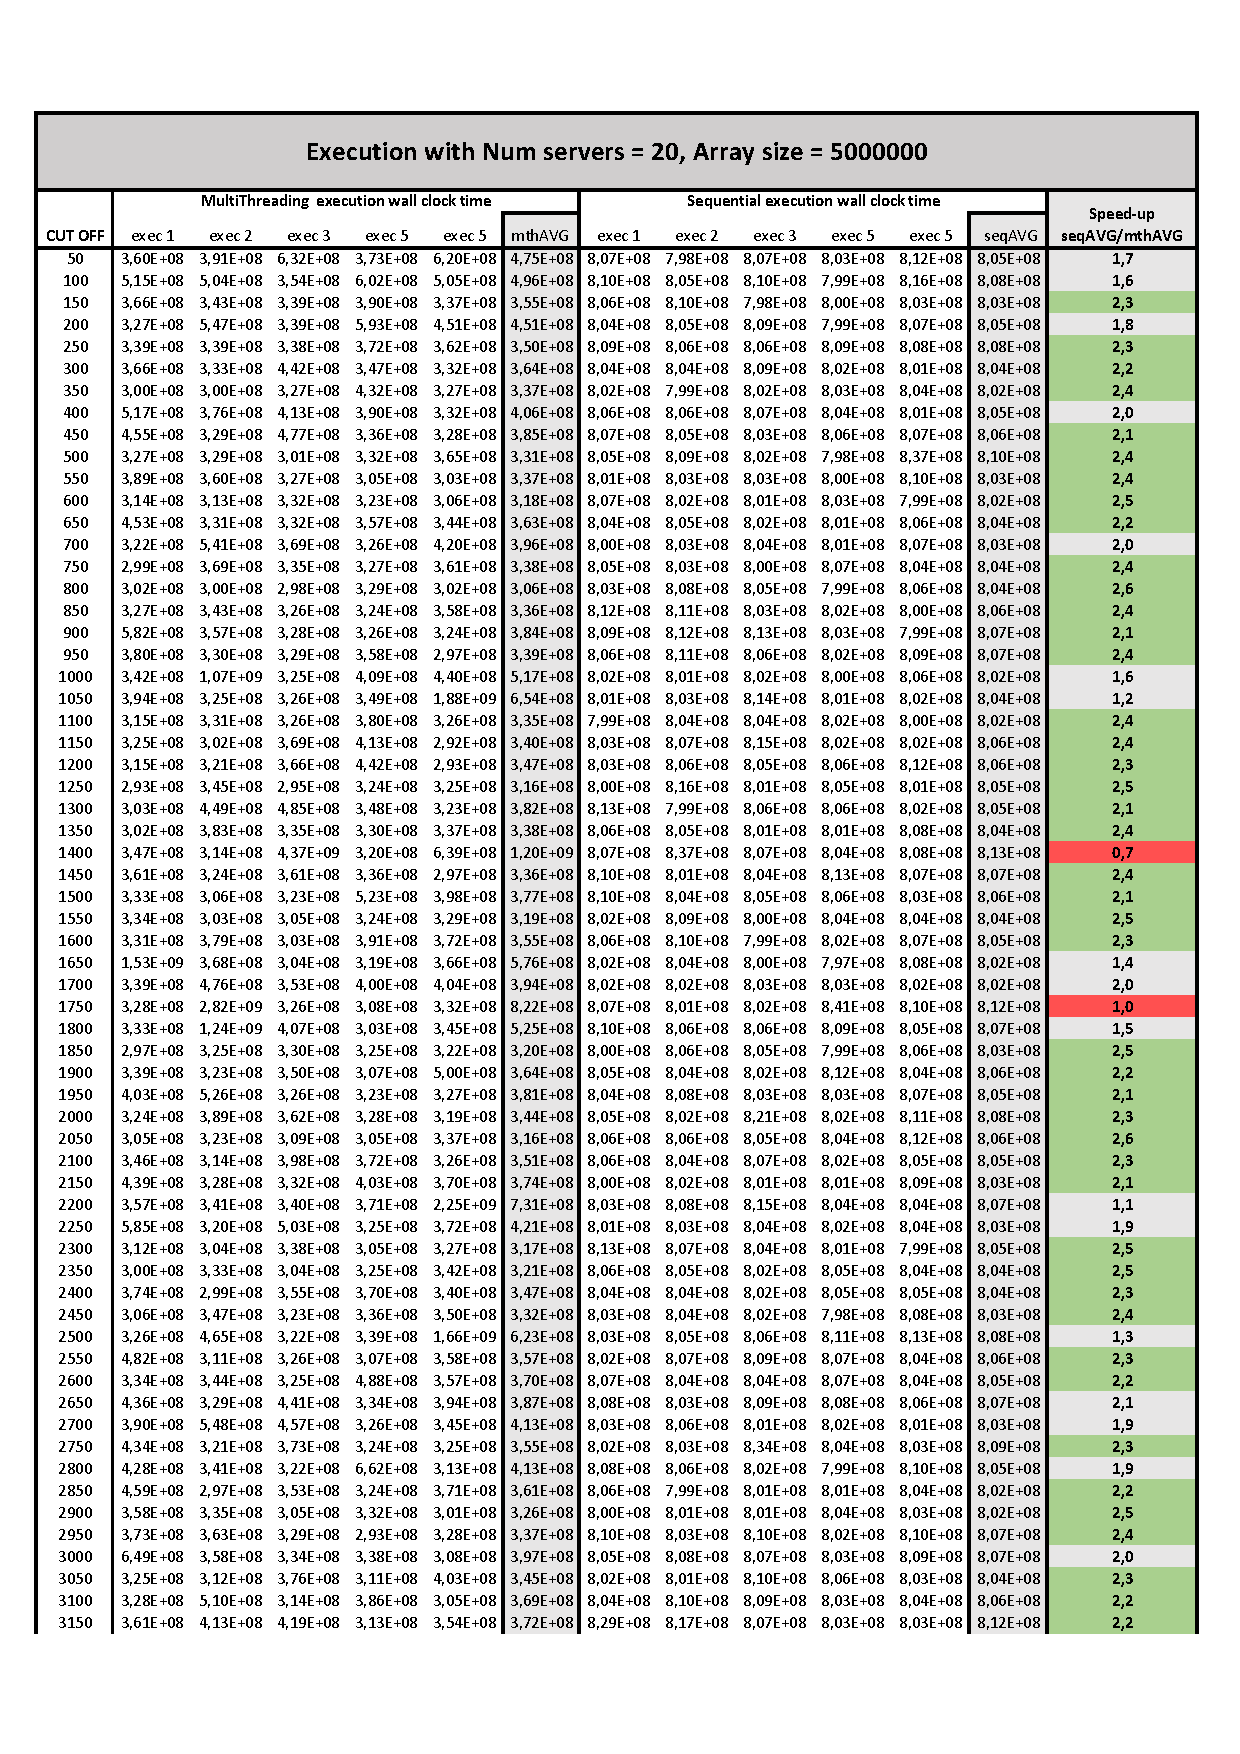
\includegraphics[page=1, width=0.9\linewidth]{imgs/CutOffAnalysis02.pdf}

\clearpage
\centering
%\hspace*{-n}
\includegraphics[page=2, width=0.9\linewidth]{imgs/CutOffAnalysis02.pdf}%
\endgroup

\clearpage 

\subsection{Further analysis}\label{CO2}
We focus on 7 different values for the cut-off and analyze the speed-up on different sizes of the array. Green cells highlight the executions in which the work stealing algorithm had a better clock-time.

\begingroup
\centering
\vspace*{-0.1in}
%\hspace*{-0.5in}
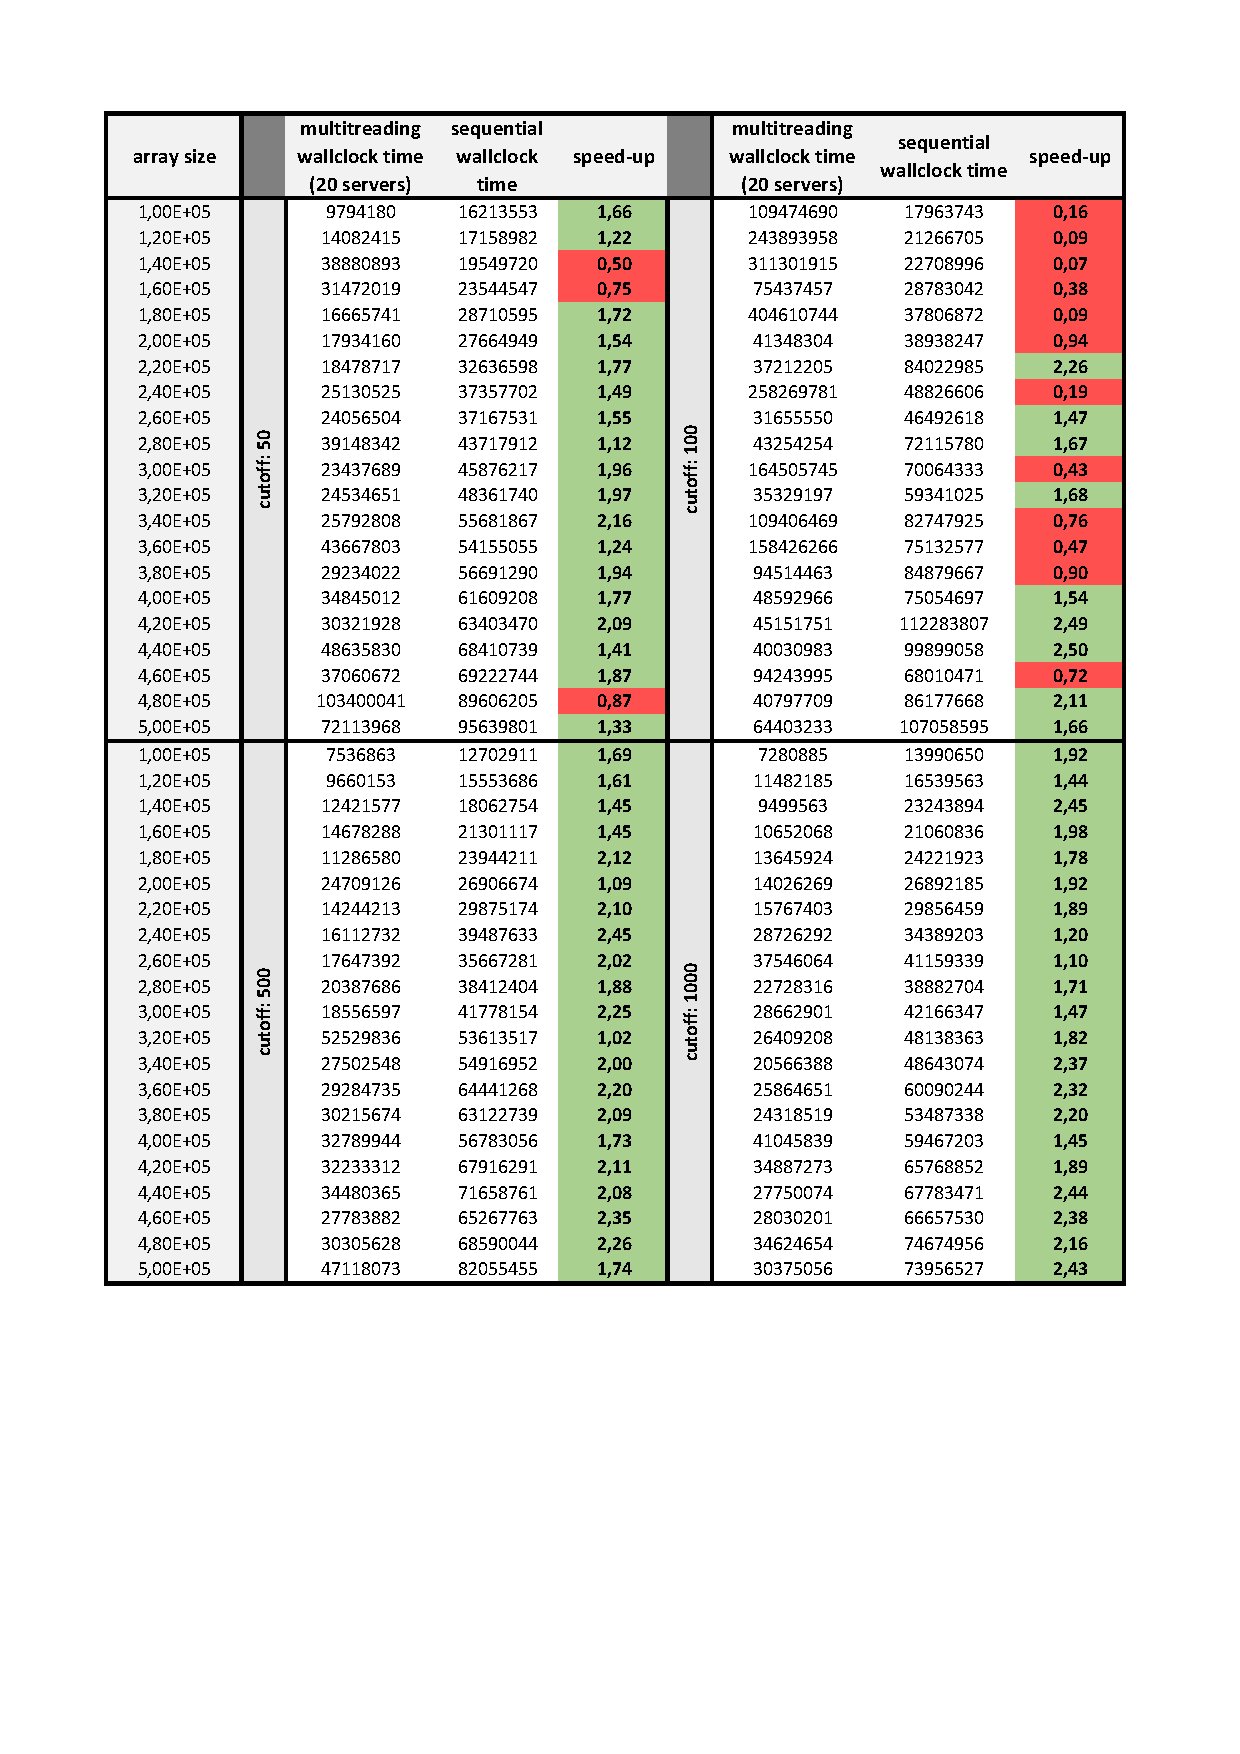
\includegraphics[page=1, width=\linewidth]{imgs/CutOff50-1000.pdf}
\endgroup

\begingroup
%\hspace*{-0.6in}
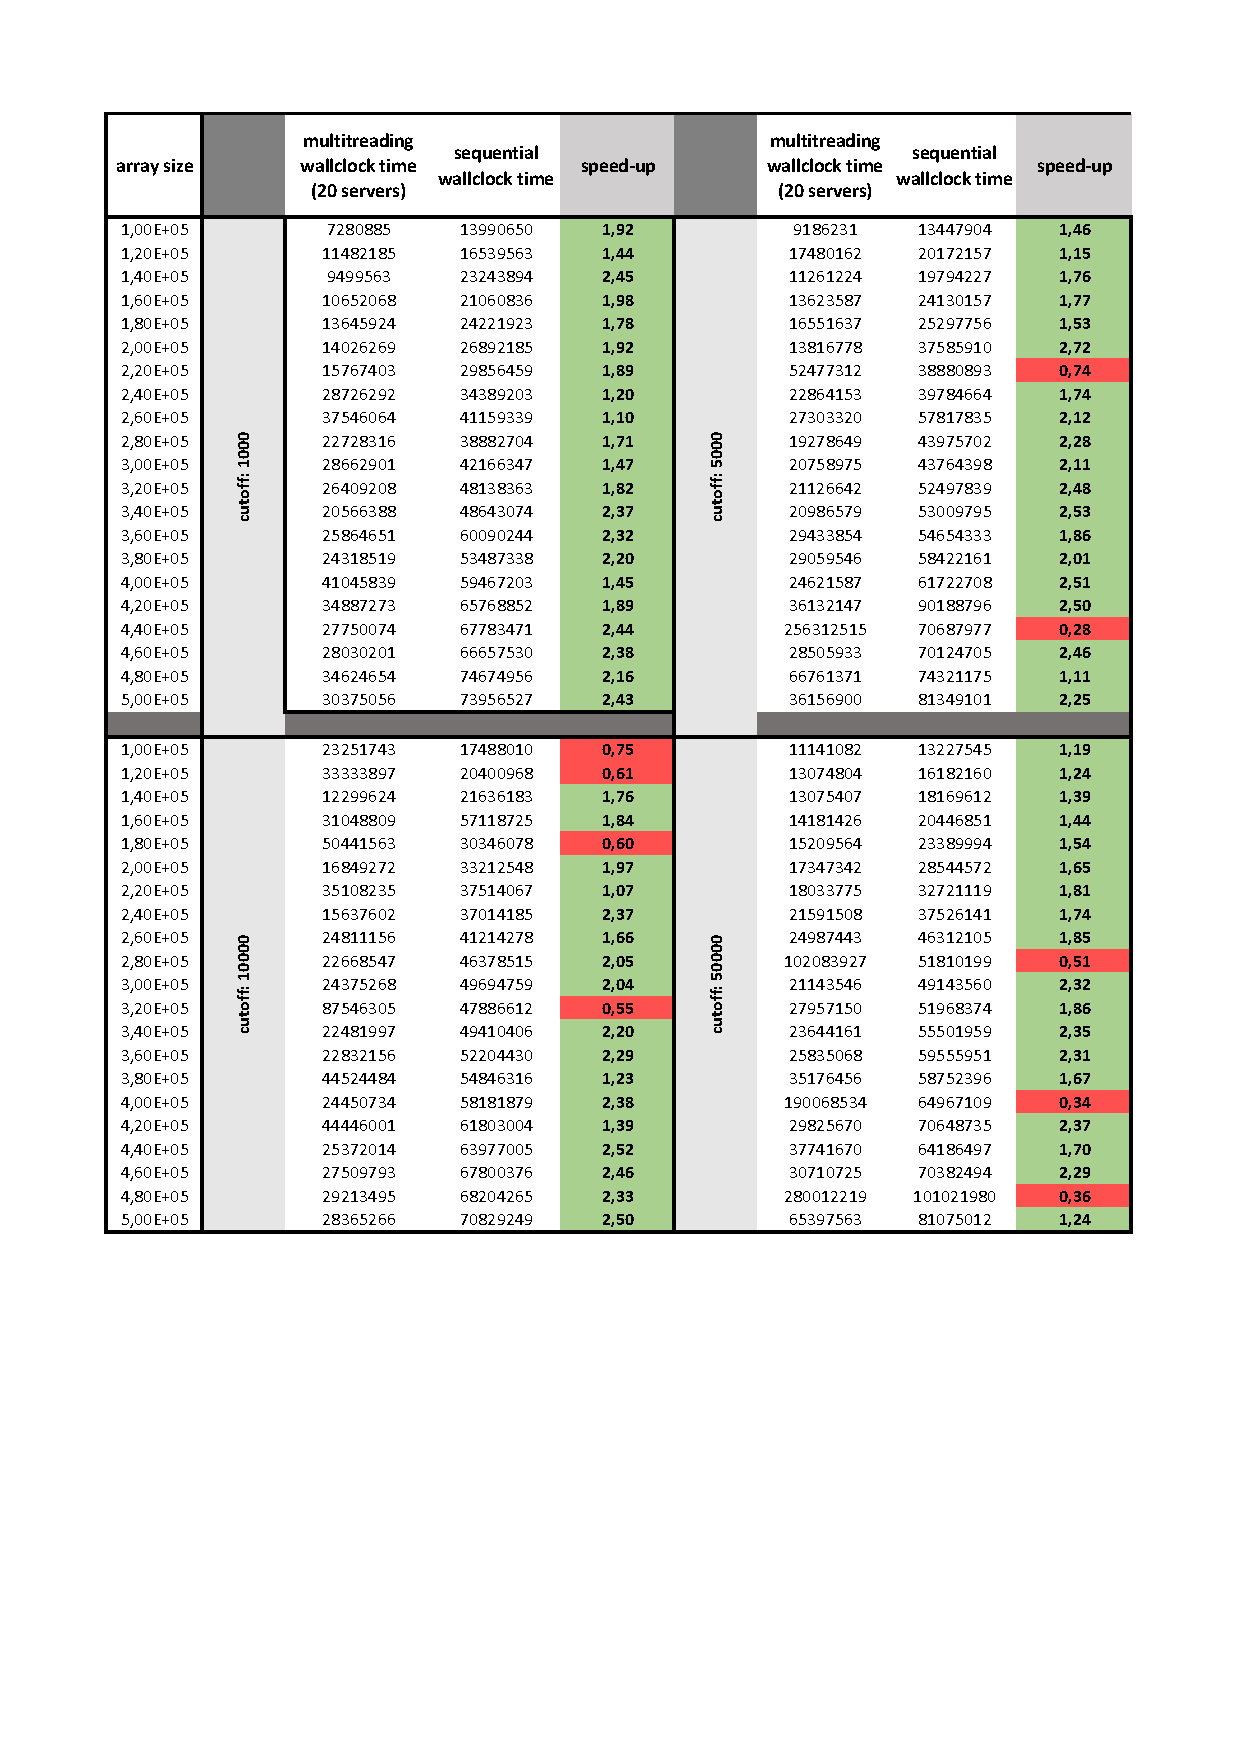
\includegraphics[page=1, width=\linewidth]{imgs/CutOff1000-5000.pdf}
\endgroup

\section{Average steals and execution time}
The table shows the average results with the size listed in the first column, 20 servers and cutoff=1000. The green cells highlight the executions in which the work stealing algorithm had a better clock-time.

\begingroup
\centering
\hspace*{-1.6in}
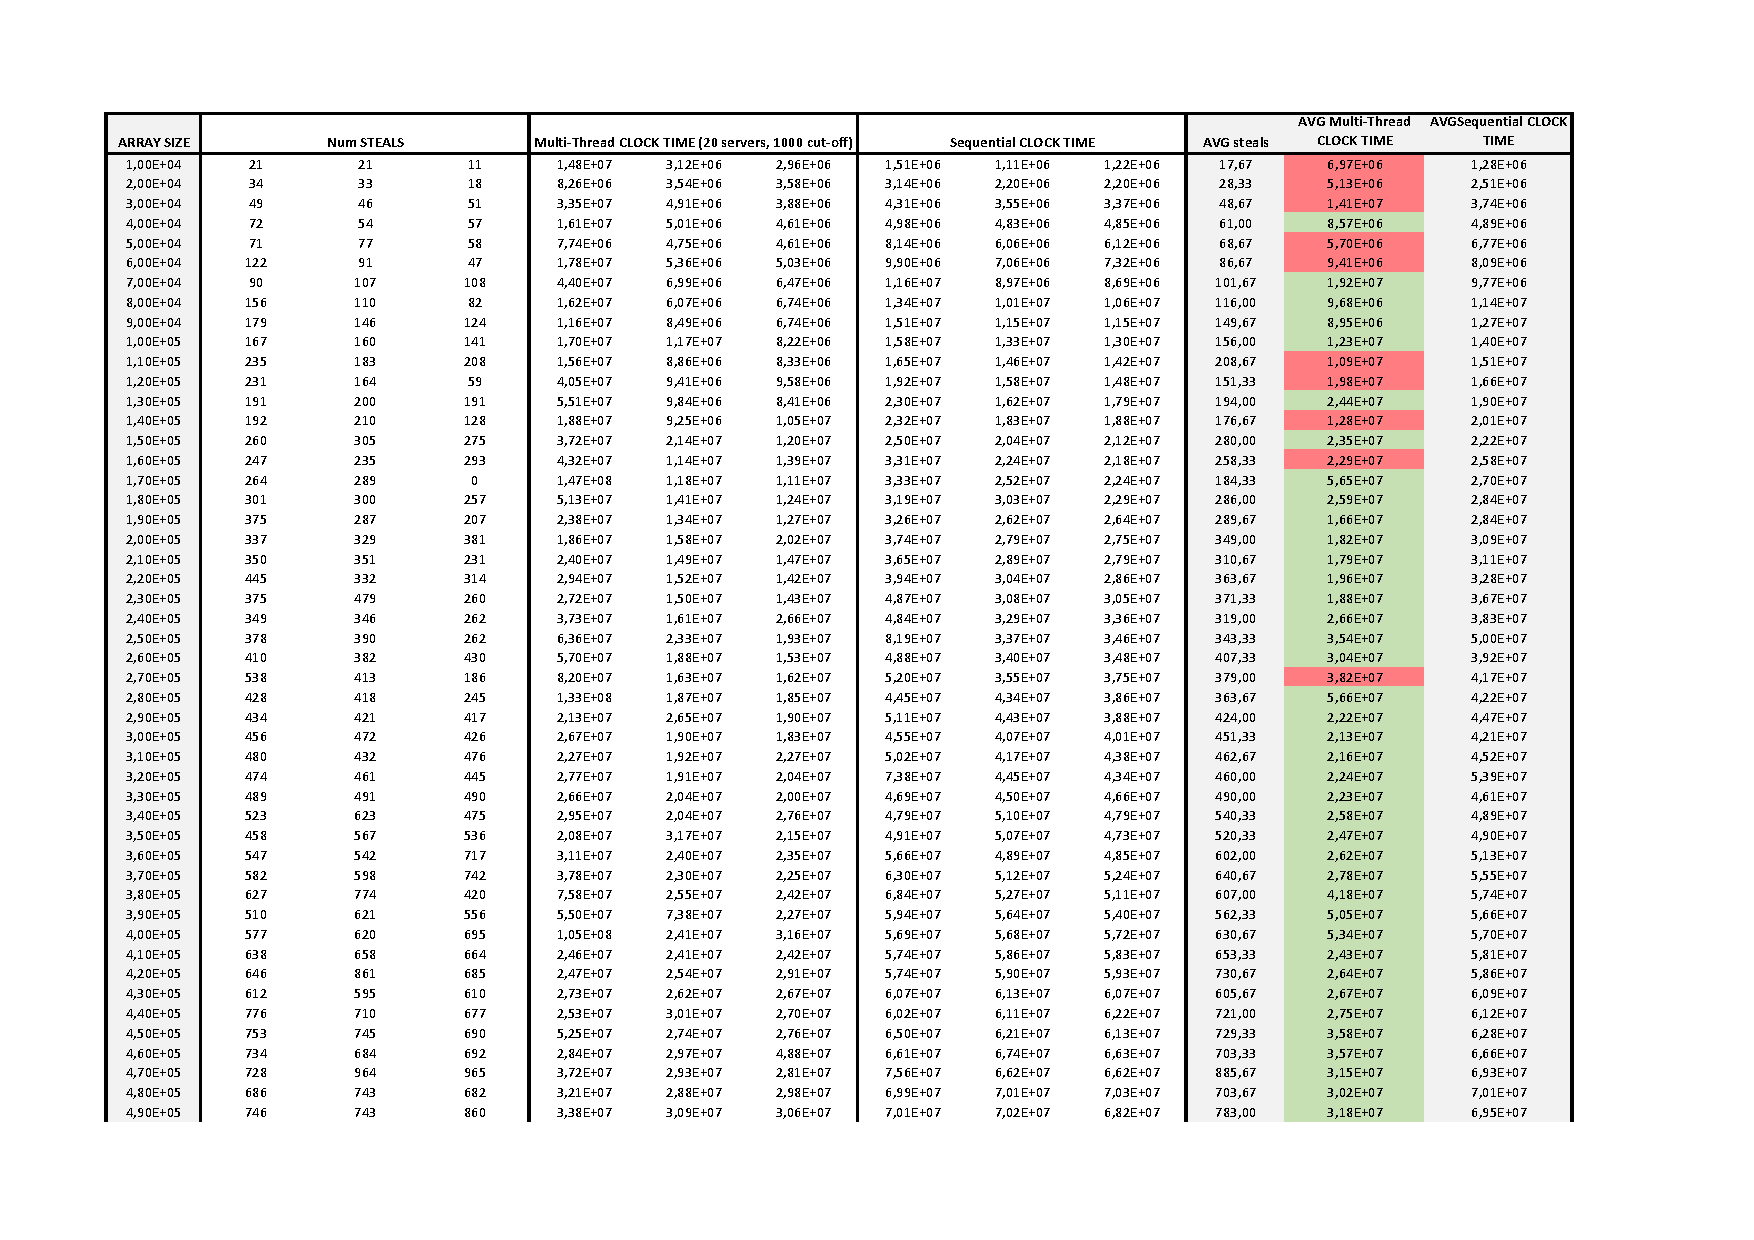
\includegraphics[page=1, width=1.6\linewidth]{imgs/steals+multithreadVSseq.pdf}
\newpage
\hspace*{-1.6in}
\includegraphics[page=2, width=1.6\linewidth]{imgs/steals+multithreadVSseq.pdf}%
\endgroup


%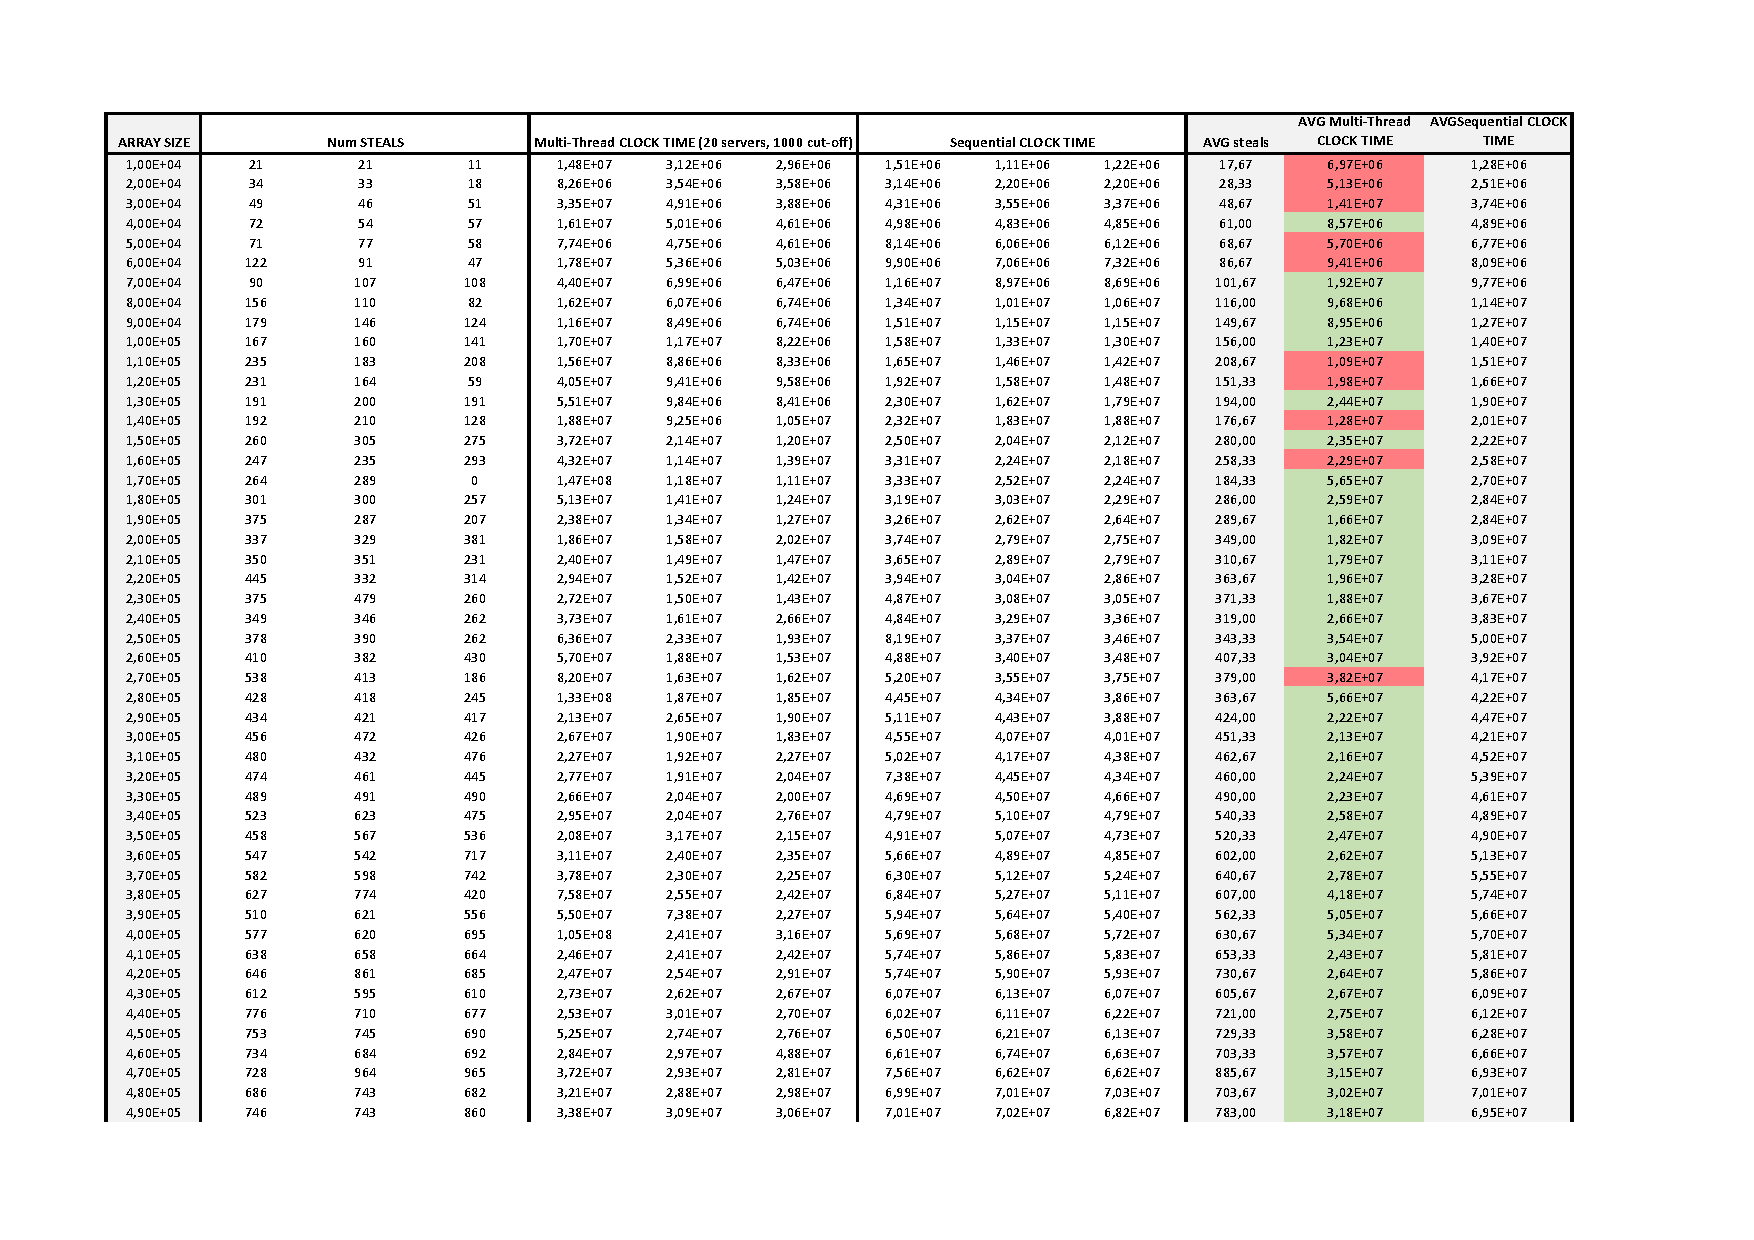
\includepdf[pages=1-2,pagecommand={\thispagestyle{plain}}]{imgs/steals+multithreadVSseq.pdf}
		
		
		% Generate the bibliography.
		%\begin{thebibliography}
		
		%\bibitem{9} Tembe, Waibhav, James Lowey, and Edward Suh. ``G-SQZ: compact encoding of genomic sequence and quality data." Bioinformatics 26.17 (2010): 2192-2194.	
		%\bibitem{10} Hach, Faraz, et al. ``SCALCE: boosting sequence compression algorithms using locally consistent encoding." Bioinformatics 28.23 (2012): 3051-3057.
		%\bibitem{11} Ochoa, Idoia, et al. ``QualComp: a new lossy compressor for quality scores based on rate distortion theory." BMC bioinformatics 14.1 (2013): 187.
		
		
		%\end{thebibliography}
		%\bibliography{latex-sample}
		%\bibliographystyle{unsrt}
	
\end{document}
